\chapter{Methodology and Implementation}
\label{chap:metodology}

Our goal with this project as outlined in \cref{chap:introduction} is creating a method for identifying LN relevant transactions on the blockchain and discover what information will be available to us by doing so. The LN is a separate network but the on-chain transactions it requires for operating channels gives us a link between the two. Because we are interested in what we can learn about the LN and its users from analyzing the blockchain, we will not utilize the information in non LN relevant transactions or users in this project. Reason behind this is the size of the blockchain as discussed in \cref{sec:related}, which means the requirements for both software and hardware will be high if all information should be kept track for parsing. The benefits of taking all information into consideration are also small four our project, however, it can be helpful and is discussed further in \cref{sec:future} on future work. 
\\

The link between the LN and the Bitcoin network will only provide us with a portion of the information about the LN and its users. By connecting to the LN itself we would have access to more information than found on the blockchain. However, the LN is a dynamic changing network of nodes, channels, and payment's; which is not stored in any public ledger like the blockchain. The information found in the LN can be recorded and stored by participants but the system itself does not keep such a record. The data in the blockchain can be verified by any user as explained in \cref{subsec:blockchain} while data recorded from the LN could not be verified in the same manner on its own.
This means that if we want historical data about the LN we must use the blockchain in which the users maintain a consensus about its correctness. Because as already stated the LN requires the Bitcoin system to operate so there will be on-chain transactions on the blockchain. We can also use the fact that there is much information available from connecting to the LN itself: collecting this information will allow us compare it with what we find on the blockchain. Doing this comparison we can verify our method for identifying LN relevant transactions on the blockchain. 

\section{Blockchain analysis}

The transactions in the blockchain is linked with outputs - inputs forming a DAG as we explained in \cref{subsec:transactions}. Parsing the blockchain would entail linking these transactions to form a transaction graph. This is necessary for applying the heuristics used by previous works discussed in \cref{sec:background}; reasion being that 

% locating relevant ln transactions

To locate LN relevant transaction we identified attributes they contained not present in other transactions. As stated in chapter 2 \todo{add ref} Lightning channels have nomrally two on-chain transactions: the founding/opening and closing transaction. This transaction pair will contain a output (found in the founding transaction) - input (found in the closing transaction) set of which is of the type P2WSH 2of2 mutlsig. This is the output - input used for the channel. This is not sufficent to determine if a transaction is related to the LN or not as P2WSH 2of2 multisig transactions can be used without any relation to the LN. If we look at an arbitrary transaction and see that it has a P2WSH output it can be a founding tx, but we dont even know if the redeem script is a 2of2 multisig script. If we see a transaction which has a single 2of2 multisig input in its redeem script, it might be a closing tx with the possibility of the preceding tx of that input being a founding tx, and that previous transaction possibility of being a founding tx is higher since we now know that the redeem script was a 2of2 multisig script. \todo{talk about 2of2 ms matching discussed later} These transactions is shown in fig.\todo{ref fig}

\begin{figure}[h]
    \centering
    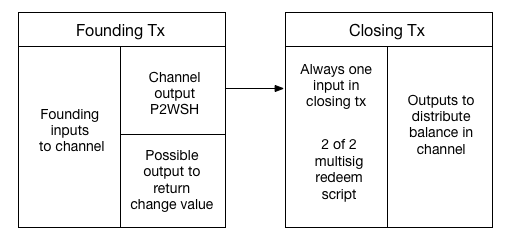
\includegraphics[width=9cm]{figures/lnchain.png}
    \caption{Algorithm of parsing and locating relevant LN transactions on the blockchain}
    \label{fig:htlc_bc}
\end{figure}

% timelocked scripts

In addition to 2of2 multisig redeem scripts there is other script types used in LN on-chain transactions. One of these scripts is the one used when a channel is unilaterally closed-i.e., one of the parties in the channel publishes a commitment transaction. As explained in section \todo{ref background} the one who publishes a commitment transaction has their output timelocked in the case of the commitment published was a revoked one with outdated balance favoring the publisher more than the most recent commitment. This means that a output of the closing/commitment transaction will be a P2WSH output with a redeem script containing the timelock, and a clause where the other party can claim the founds if the it was an old commitment they therefore have the revocation key. This transaction chain is shown in fig \todo{ref fig}

\begin{figure}[h]
    \centering
    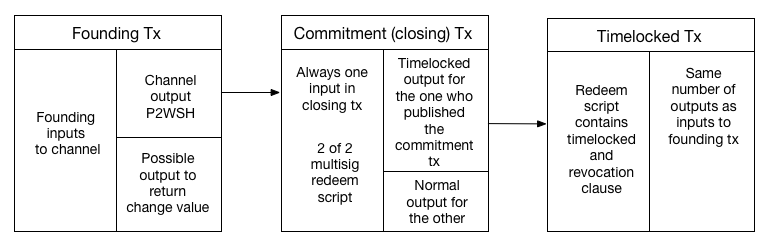
\includegraphics[width=12cm]{figures/lnchainTimelock.png}
    \caption{Algorithm of parsing and locating relevant LN transactions on the blockchain \todo{fix fig, it is wrong}}
    \label{fig:htlc_bc}
\end{figure}

This redeem script is fairly unique and to our knowledge there is no other instances such scripts are used. However, people are free to create such scripts without it having anything to do with the LN the specific use case of such script makes this unlikely. Since the redeem script is located in the transaction spending the P2WSH output we need to identify it in the transaction spending the timelocked tx shown in fig \todo{ref fig over}. Since transactions have references to previous transaction hashes \todo{check if transaction hashes is explaned in bckground} we can by finding the transaction spending a timelocked output get the hash of the timelocked tx. When we have the timelocked tx it will contain the hash of the input tx, and this will again allow us to find the tx hash of the closing tx which will in turn give us the founding tx. Doing this will result in us finding all on-chain transactions related to a unilatirally closed lightning channels.

This method identify the transactions related to a lightning channel in reverse order meaning the transaction spending the timelocked output will be indentified first and the founding transaction last. 
This means we must parse the blockchain in reverse order starting from the lastest block working our way down the the start; the structure of the blockchain with blocks only contain the hash of the previous block is another reason for this.
For this project we have developed software parsing the blockchain and identified relevant transaction as outlined above.
At a high level the software finds the top block from the chaindata stored in the database and uses it as a starting point.
Then it traverses the transactions in the block and checks if they are relevant for our project, if that is the case they are stored for later use. The hash of the preceding block is used to get it from the database and same process is repeated.
The algorithm used is based on identifying scripts from the timelocked output of a unilatirally closed channel, and then using the transaction hash of the previous transaction to get the rest of the relevant channels as shown in fig. \todo{add ref fig}

\begin{figure}[h]
    \centering
    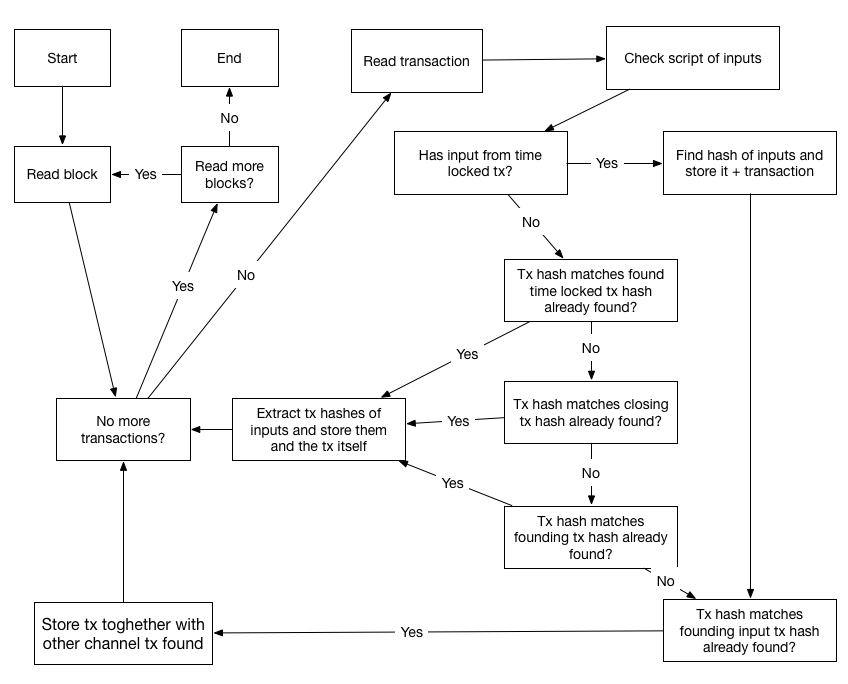
\includegraphics[width=14cm]{figures/algorithm.png}
    \caption{Algorithm of parsing and locating relevant LN transactions on the blockchain}
    \label{fig:htlc_bc}
\end{figure}

% ln transaction formats on chain

When a transaction is inspected we first check if it has a input containing a redeem script for a timelocked transaction.
The script is defined in the lightning rfc \todo{add ref to rfc} and has the format:
\\

\noindent OP\_IF \\
    # Penalty transaction \\
    <revocationpubkey> \\
OP\_ELSE\\
    `to\_self\_delay`\\
    OP\_CSV\\
    OP\_DROP\\
    <local\_delayedpubkey>\\
OP\_ENDIF\\
OP\_CHECKSIG\\

The first line is the clause to stop participants from publishing old commitment transactions. The script will evaluate to true if this clause is used and the signature for the public key is given; As discussed in section \todo{ref bacground} the parties will revoke old commitment transactions by exchanging keys so the other party can spend the timelocked output with the revocation key and get all the founds in the channel. The else clause is the timelocked portion of the script; it will contain a delay and the CHECKSEQUENCEVERIFY operation defined in \todo{ref bip 112} which terminates the script if the delay has not passed. The delay is then removed from the stack with OP\_DROP such that the signature and public key are the only two items on the stack when OP\_CHECKSIG is used to very the signature.

% identifying scripts in depth

% multisig detection

% how other information gathered. output types so on.

\section{Lightning network analysis}

% lnd introduction

%why gather ln data (relate to background and goals)

%how ln data was gathered

To gather data from the LN we used a modified version of the LND \todo{add ref} implementation, which follows the BOLT specification \todo{add ref}. It maintains a view of the network by storing a graph containing active channels. This is continuously updated as new channels are annouched and closing transactions is found on the blockchain. It requires a bitcoin backend running to interact with the bitcoin network; using it to publish on-chain transactions and monitor the blockchain. New channels are discovered by annouchements within the LN while channels closing is found by looking at the blockchain and finding transactions spending the founding transactions of previously active channels. We forked and modifed LND to create a copy of its database each time a new block notification was received from the Bitcoin software giving us a snapshot of the network on each new block.
\\

Each snapshot we collected contained the graph describing the network in its current state, so by comparing the graphs of different snapshorts we can see how the network evolves over time. When comparing two snapshots from two points in time we can identify closed channels by checking the old snapshot for channels not found in the new one; Similarly new channels can be found by checking the new snapshot for channels not found in the old one. This allows us to build a list of closed and opened channels during the collection timeframe, as well as the those which are open throughout. 

% details getting channels.

\section{Clustering}

% intro clusting, goals and related work

% how we cluster channels and so on.